\section{Layout}

Com os resultados de simulação validando o funcionamento do circuito, foi possível iniciar o desenvolvimento do layout. Todo o projeto foi realizado utilizando a ferramenta \textit{Virtuoso}, da \textit{Cadence}, utilizando o processo \textit{TSMC CMOS 180 nm}. O circuito integrado apresentado na \autoref{fig_circintegrado} foi desenvolvido, contendo todo o projeto de Receptor Óptico além de outros projetos desenvolvido por outros alunos\footnote{"Projeto de um Oscilador em Anel Controlado por Tensão de Múltiplas Saídas em Tecnologia CMOS 180 nm" \cite{VictorRodrigues}}\footnote{"Projeto de um Conversor CC-CC CMOS para Aplicações de Energy Harvesting" \cite{LucasChaves}}. A \autoref{fig_circintegrado_division} mostra de maneira explicita o que representa cada parte do CI. O circuito integrado apresenta uma área total de 2x2 mm² (2,56 mm²), utilizando um encapsulamento do tipo CLCC44\footnote{Especificações do encapsulamento presentes no \autoref{anexo_clcc44}}. A \autoref{tab_clcc44} apresenta a relação da numeração dos pinos do encapsulamento com os pinos chip, que são distintos, além da identificação de cada pino.

\begin{figure}[htb]
 \centering
    \caption{Circuito Integrado utilizado para o Receptor Óptico} 
    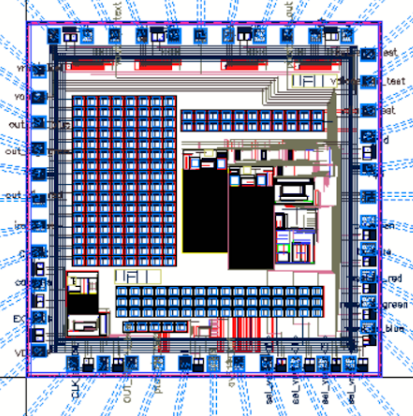
\includegraphics[scale=0.5]{Resultados/Imagens/CircuitoIntegrado.png}
    \legend{Fonte: Produzido pelo autor}
    \label{fig_circintegrado}
\end{figure}

\begin{figure}[htb]
 \centering
    \caption{Circuito Integrado utilizado para o Receptor Óptico particionado} 
    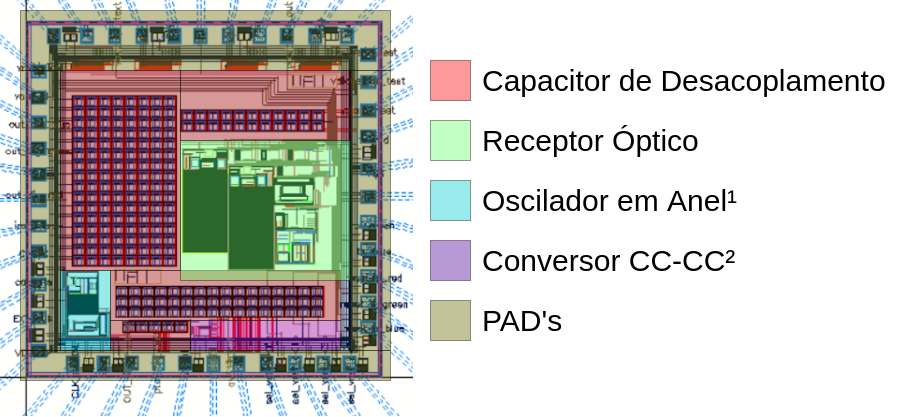
\includegraphics[scale=0.5]{Resultados/Imagens/Image_CircuitoIntegrado.png}
    \legend{Fonte: Top View desenvolvido por Daniel Carvalho Lott}
    \label{fig_circintegrado_division}
    \nota{¹ Projeto desenvolvido por Victor Rodrigues Barbosa \cite{VictorRodrigues}\\² Projeto desenvolvido por Lucas Martins Chaves \cite{LucasChaves}}
\end{figure}

A \autoref{layoutcompleto} apresenta a implementação completa do Receptor Óptico projetado. A \autoref{layoutcompleto_division} mostra a mesma figura explicitando o que representa as diferentes parte do circuito. O projeto do Receptor Óptico ocupa uma área de X um².

\begin{figure}[htb]
 \centering
    \caption{Layout completo do circuito desenvolvido} 
    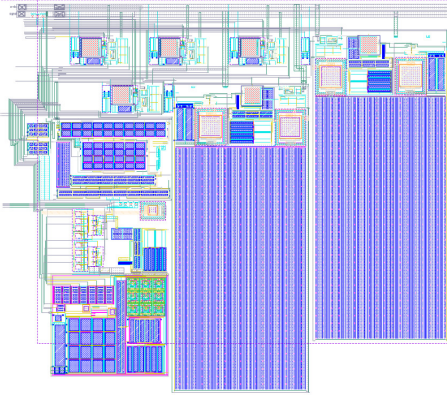
\includegraphics[scale=1, angle = 90]{Resultados/Imagens/Circuito Completo.png}
    \legend{Fonte: Produzido pelo autor}
    \label{layoutcompleto}
    \nota{Imagem rotacionada em 90° em sentido anti-horário}
\end{figure}

\begin{figure}[htb]
 \centering
    \caption{Layout completo do circuito particionado} 
    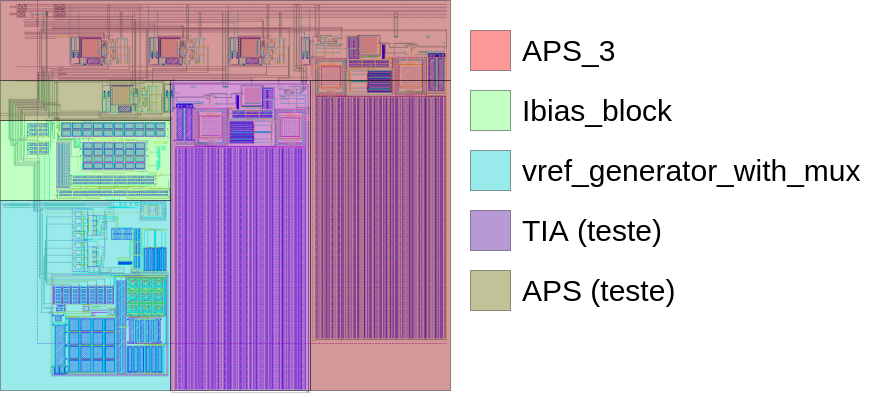
\includegraphics[scale=0.3]{Resultados/Imagens/Image_CircuitoCompleto.png}
    \legend{Fonte: Produzido pelo autor}
    \label{layoutcompleto_division}
\end{figure}

O bloco \textit{APS\_digitalized} projetado é apresentado na figura \autoref{layoutAPSDIG}. A \autoref{layoutAPSDIG_division} mostra a mesma figura explicitando o que representa as diferentes parte do circuito. O projeto do bloco ocupa uma área de X um², tendo X um de altura e X um de comprimento.

\begin{figure}[htb]
 \centering
    \centering
    \caption{Layout do bloco \textit{APS\_digitalized}} 
    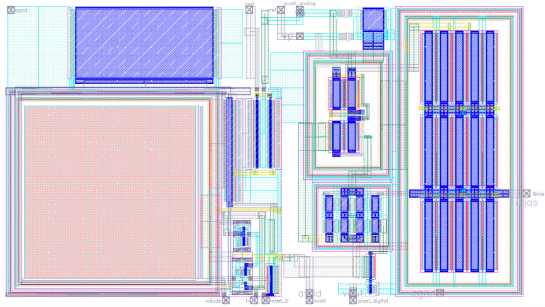
\includegraphics[scale=0.8]{Resultados/Imagens/APS_DIGITALIZED.png}
    \legend{Fonte: Produzido pelo autor}
    \label{layoutAPSDIG}
\end{figure}

\begin{figure}[htb]
 \centering
    \centering
    \caption{Layout do bloco \textit{APS\_digitalized} particionado} 
    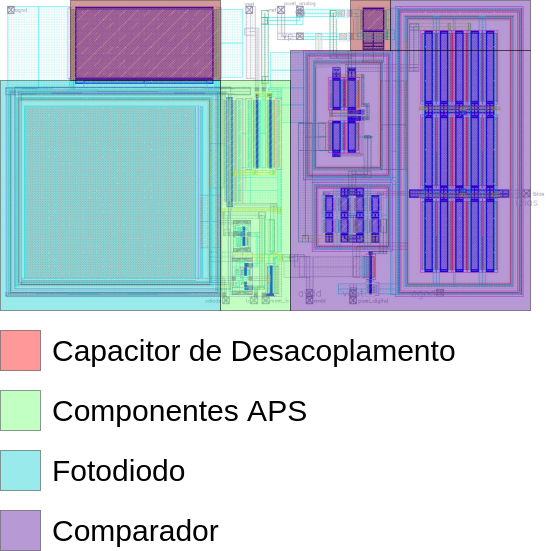
\includegraphics[scale=0.3]{Resultados/Imagens/Image_APS_Digitalized.png}
    \legend{Fonte: Produzido pelo autor}
    \label{layoutAPSDIG_division}
\end{figure}

O bloco \textit{APS\_clk} projetado é apresentado na figura \autoref{layoutTIA}. A \autoref{layoutTIA_division} mostra a mesma figura explicitando o que representa as diferentes parte do circuito. O projeto do bloco ocupa uma área de X um², tendo X um de altura e X um de comprimento.

\begin{figure}[htb]
 \centering
    \centering
    \caption{Layout do bloco \textit{APS\_clk}} 
    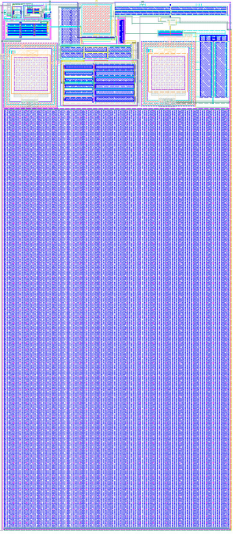
\includegraphics[scale=0.7]{Resultados/Imagens/TIA.png}
    \legend{Fonte: Produzido pelo autor}
    \label{layoutTIA}
\end{figure}

\begin{figure}[htb]
 \centering
    \centering
    \caption{Layout do bloco \textit{APS\_clk} particionado}
    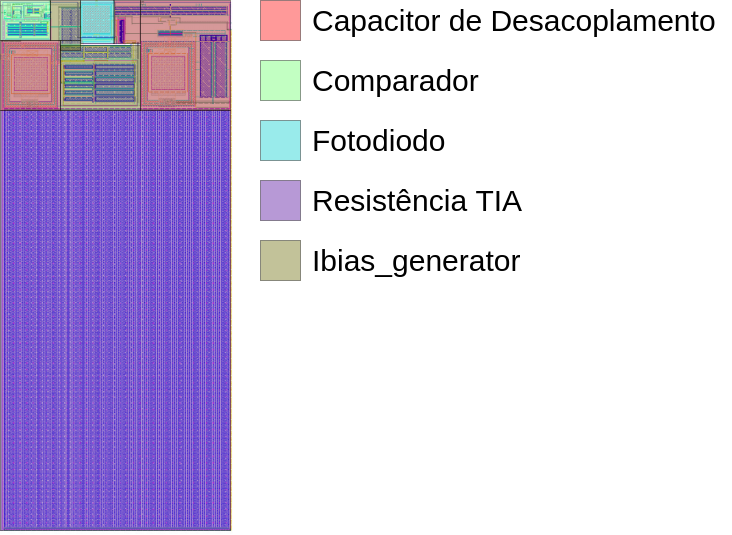
\includegraphics[scale=0.3]{Resultados/Imagens/Image_TIA.png}
    \legend{Fonte: Produzido pelo autor}
    \label{layoutTIA_division}
\end{figure}

O bloco \textit{APS\_3} projetado é apresentado na figura \autoref{layoutAPS_3}. A \autoref{layoutAPS_3_division} mostra a mesma figura explicitando o que representa as diferentes parte do circuito. O projeto do bloco ocupa uma área de X um², tendo X um de altura e X um de comprimento.

\begin{figure}[htb]
 \centering
    \centering
    \caption{Layout do bloco \textit{APS\_3}} 
    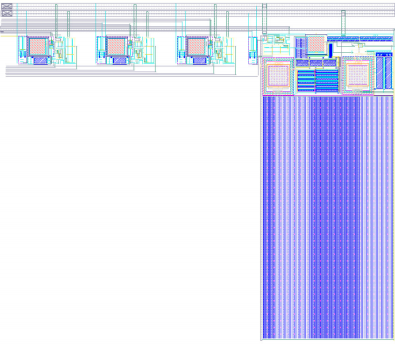
\includegraphics[scale=0.8]{Resultados/Imagens/APS_3.png}
    \legend{Fonte: Produzido pelo autor}
    \nota{Imagem do circuito rotacionado em 90° em relação à orientação padrão do circuito no plano (1 1 0).}
    \label{layoutAPS_3}
\end{figure}

\begin{figure}[htb]
 \centering
    \centering
    \caption{Layout do bloco \textit{APS\_3} particionado} 
    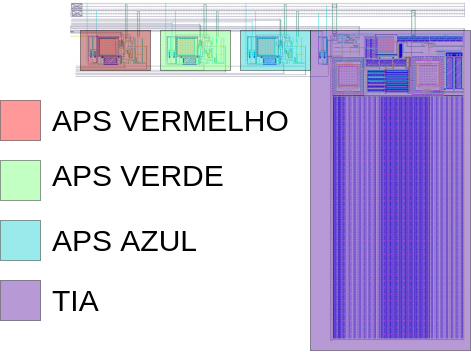
\includegraphics[scale=0.3]{Resultados/Imagens/Image_APS_3.png}
    \legend{Fonte: Produzido pelo autor}
    \label{layoutAPS_3_division}
\end{figure}
